\documentclass[border=3pt]{standalone}
% Preâmbulo compartilhado pelos diagramas TikZ da aula 8 de IHC (Design de IHC)
\usepackage[T1]{fontenc}
\usepackage[utf8]{inputenc}
\usepackage{lmodern}
\usepackage{amsmath}
\usepackage{xcolor}
\usepackage{tikz}
\usetikzlibrary{arrows.meta,angles,quotes,decorations.pathmorphing,decorations.pathreplacing,calc,
                positioning,shapes.geometric,shapes.misc,backgrounds,fit,
                math}

% Paleta (mesma dos SVGs originais)
% Paleta da disciplina de IHC: acento roxo (#755099), da capa do livro.
% (o nome "dblue" é mantido para não alterar todos os diagramas)
\definecolor{dblue}{HTML}{755099}
\definecolor{dorange}{HTML}{B3541E}
\definecolor{dgreen}{HTML}{4A7C59}
\definecolor{dred}{HTML}{9C4B4B}
\definecolor{dcream}{HTML}{F4F1EA}
\definecolor{dshade}{HTML}{DDD7C9}

% Função gaussiana (não normalizada por padrão de escala visual)
\pgfmathdeclarefunction{gauss}{3}{%
  \pgfmathparse{1/(#3*sqrt(2*pi))*exp(-((#1-#2)^2)/(2*#3^2))}%
}

% Estilos comuns (prefixo d... para não colidir com chaves internas do pgf)
\tikzset{
  >={Stealth[length=2mm]},
  dguide/.style={gray!55, dashed, line width=0.4pt},
  daxis/.style={gray!60, line width=0.7pt, ->},
  dbody/.style={fill=black!3, draw=black!80, line width=1pt},
  dacc/.style={draw=dblue, line width=1pt},
  dlbl/.style={black!55, font=\small},
  dsub/.style={black!45, font=\footnotesize},
  dstate/.style={circle, draw=black!80, fill=dcream, line width=1pt,
                 minimum size=17mm, font=\large, inner sep=1pt},
  dobs/.style={circle, draw=black!80, fill=dshade, line width=1pt,
               minimum size=14mm, font=\large, inner sep=1pt},
  dbox/.style={rounded corners=2pt, draw=black!80, fill=dcream, line width=1pt,
               align=center, inner sep=6pt},
  dop/.style={circle, draw=black!80, fill=white, line width=1pt,
              minimum size=6mm, inner sep=0pt, font=\small},
  dtrans/.style={->, dblue, line width=1pt},
  dmeas/.style={->, dorange, line width=1pt},
  dcurve/.style={line width=1pt, dblue},
  dcurveb/.style={line width=1.4pt, dorange},
}

\begin{document}
\hyphenpenalty=10000 \exhyphenpenalty=10000 \tolerance=9999 \emergencystretch=3em
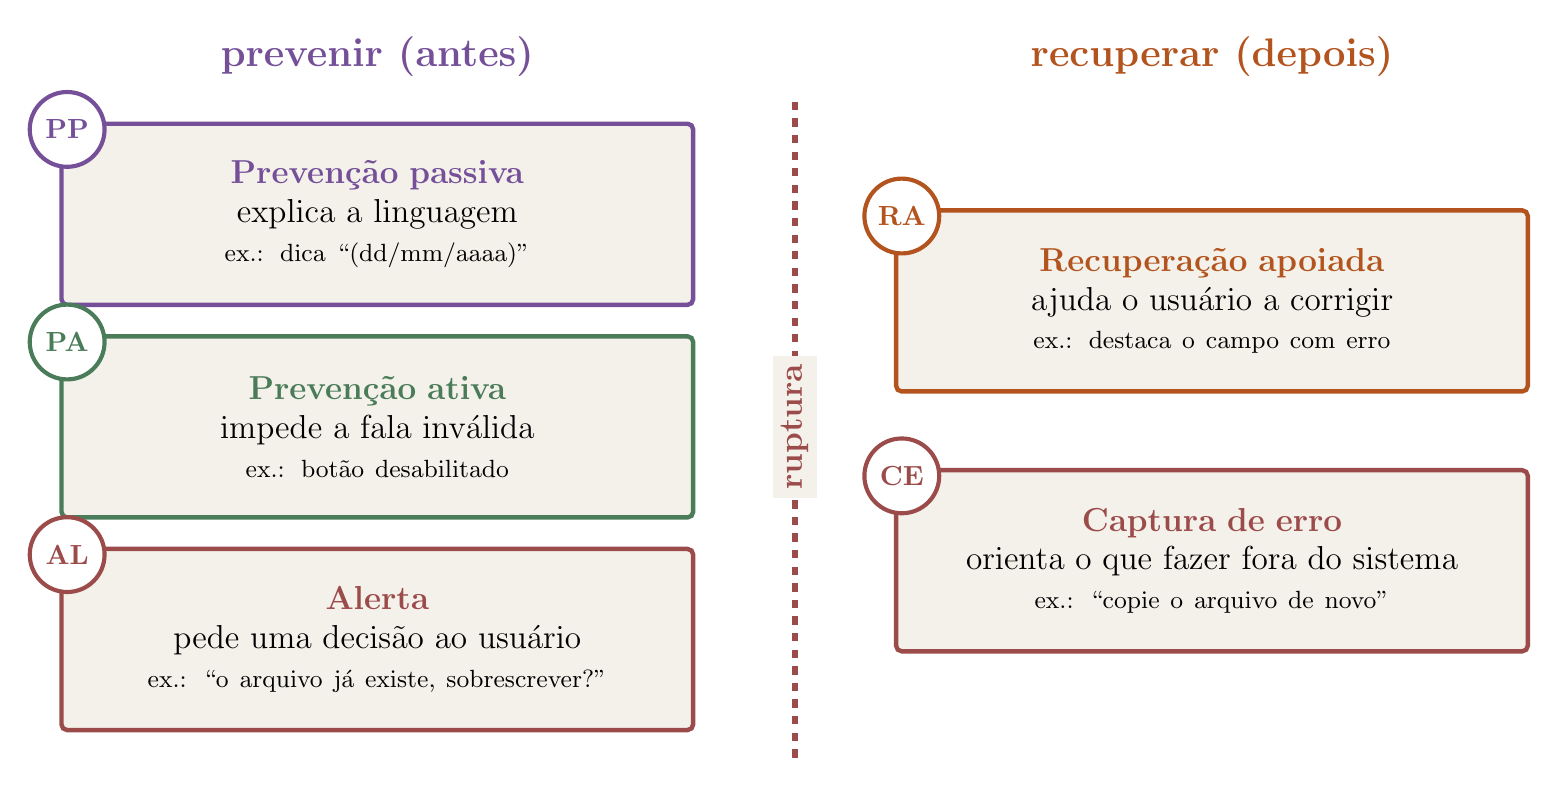
\begin{tikzpicture}[x=1cm,y=1cm]
\tikzset{c/.style={dbox, text width=7.6cm, minimum height=2.3cm, font=\large, line width=1.6pt},
        sg/.style={circle, fill=white, line width=1.5pt, font=\normalsize\bfseries, inner sep=1pt, minimum size=0.95cm}}
\node[font=\Large\bfseries, dblue] at (4.4,9.3) {prevenir (antes)};
\node[font=\Large\bfseries, dorange] at (15.0,9.3) {recuperar (depois)};
\node[c, draw=dblue] (pp) at (4.4,7.3) {\textbf{\textcolor{dblue}{Prevenção passiva}}\\ explica a linguagem\\ \small ex.: dica ``(dd/mm/aaaa)''};
\node[c, draw=dgreen] (pa) at (4.4,4.6) {\textbf{\textcolor{dgreen}{Prevenção ativa}}\\ impede a fala inválida\\ \small ex.: botão desabilitado};
\node[c, draw=dred] (al) at (4.4,1.9) {\textbf{\textcolor{dred}{Alerta}}\\ pede uma decisão ao usuário\\ \small ex.: ``o arquivo já existe, sobrescrever?''};
\draw[dred, dashed, line width=2.2pt] (9.7,0.4) -- (9.7,8.8);
\node[font=\large\bfseries, dred, fill=dcream, inner sep=3pt, rotate=90] at (9.7,4.6) {ruptura};
\node[c, draw=dorange] (ra) at (15.0,6.2) {\textbf{\textcolor{dorange}{Recuperação apoiada}}\\ ajuda o usuário a corrigir\\ \small ex.: destaca o campo com erro};
\node[c, draw=dred] (ce) at (15.0,2.9) {\textbf{\textcolor{dred}{Captura de erro}}\\ orienta o que fazer fora do sistema\\ \small ex.: ``copie o arquivo de novo''};
\node[sg, draw=dblue, text=dblue] at ($(pp.north west)+(0.1,-0.1)$) {PP};
\node[sg, draw=dgreen, text=dgreen] at ($(pa.north west)+(0.1,-0.1)$) {PA};
\node[sg, draw=dred, text=dred] at ($(al.north west)+(0.1,-0.1)$) {AL};
\node[sg, draw=dorange, text=dorange] at ($(ra.north west)+(0.1,-0.1)$) {RA};
\node[sg, draw=dred, text=dred] at ($(ce.north west)+(0.1,-0.1)$) {CE};
\end{tikzpicture}
\end{document}
